% Shared styles for the TCDS diagrams (colours as in the plots: child blue, caregiver orange,
% learned coupling green, ink greys).
\usepackage{mathptmx}
\usepackage{amsmath}
\usepackage{graphicx}
\graphicspath{{../figures/}{figures/}}
\usetikzlibrary{positioning,fit,arrows.meta,backgrounds,calc,decorations.pathreplacing}
\definecolor{child}{HTML}{2A78D6}
\definecolor{carer}{HTML}{EB6834}
\definecolor{coupling}{HTML}{1BAF7A}
\definecolor{ink}{HTML}{0B0B0B}
\definecolor{muted}{HTML}{52514E}
\definecolor{faint}{HTML}{B9B8B2}
\tikzset{
  >={Stealth[length=2mm]},
  box/.style={draw=#1, fill=#1!9, rounded corners=2pt, line width=0.8pt, align=center,
              inner sep=3pt, text=ink},
  osc/.style={box=#1, minimum width=2.3cm, minimum height=0.9cm},
  model/.style={osc=#1, dashed, fill=#1!4},
  coup/.style={box=coupling, minimum height=0.62cm},
  plain/.style={box=muted, fill=white, line width=0.6pt},
  frame/.style={draw=#1, rounded corners=4pt, line width=0.9pt, inner sep=5pt},
  arr/.style={->, line width=0.7pt, draw=muted},
  darr/.style={<->, line width=0.7pt, draw=muted},
  note/.style={font=\scriptsize, text=muted, align=center},
  ptitle/.style={font=\small\bfseries, text=ink, anchor=west},
}
% \miro{position}{colour}{label}: the MiRo-E photograph with a coloured label underneath
\newcommand{\miro}[3]{%
  \node[inner sep=0pt] at #1 {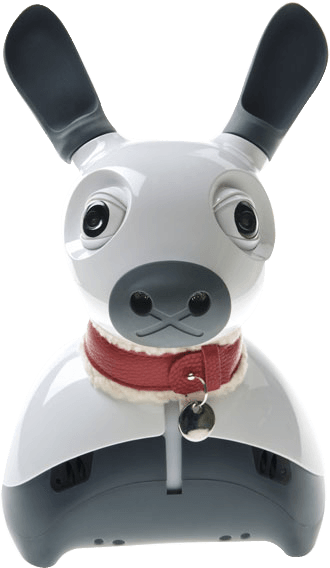
\includegraphics[height=1.05cm]{miro.png}};
  \node[font=\scriptsize\bfseries, text=#2, anchor=north] at ($#1+(0,-0.55)$) {#3};}
% \robot{position}{colour}{label}: a small stylised MiRo seen from the side
\newcommand{\robot}[3]{%
  \begin{scope}[shift={#1}]
    \draw[#2, line width=0.6pt] (-0.42,0.04) .. controls (-0.58,0.10) .. (-0.62,0.27);
    \filldraw[draw=#2, fill=#2!15, line width=0.6pt] (0,0) ellipse (0.43 and 0.23);
    \filldraw[draw=#2, fill=#2!15, line width=0.6pt] (0.40,0.22) circle (0.16);
    \fill[#2] (0.31,0.35) -- (0.27,0.50) -- (0.38,0.38) -- cycle;
    \fill[#2] (0.44,0.37) -- (0.48,0.52) -- (0.53,0.35) -- cycle;
    \fill[#2] (0.47,0.24) circle (0.025);
    \fill[#2] (-0.18,-0.24) circle (0.07);
    \fill[#2] (0.18,-0.24) circle (0.07);
    \node[note, text=ink, below=0.3cm] at (0,0) {#3};
  \end{scope}}
